The following sections describe preliminary experiments conducted to assess the feasibility of the proposed vision framework.
The experiments' primary focus is on the first stage \emph{S1}, as it is the foundation to develop the second stage \emph{S2}. Furthermore, no work exists about implementing stage \emph{S1}, in contrast to self-organising projection fibres, which are the central element of \emph{S2}.
However, to demonstrate the effectiveness of incorporating feedback from the second into the first stage, a simple mockup is used to simulate \emph{S2}.

In the remainder of this chapter, a simple dataset is introduced in \secref{exp_dataset}. Next, the implementation of the sensory system is presented in \secref{exp_s0}, the feature extracting stage in \secref{exp_s1}, and the prototype stage in \secref{exp_s2}. The results obtained from these experiments are presented in \chref{results}.


\section{Dataset}\seclbl{exp_dataset}
The objective of the experiments conducted is to demonstrate that building net fragments can be implemented using Hebbian learning \sidecite{hebb_organization_1949} (c.f. \secref{hebbian}).
Thereby, the focus is on researching novel principles and comprehending and analysing the networks' output rather than scaling the model to large datasets or pushing benchmarks.
Consequently, a straightforward dataset is introduced that comprises straight lines only.


\begin{figure}[h]
    \centering
    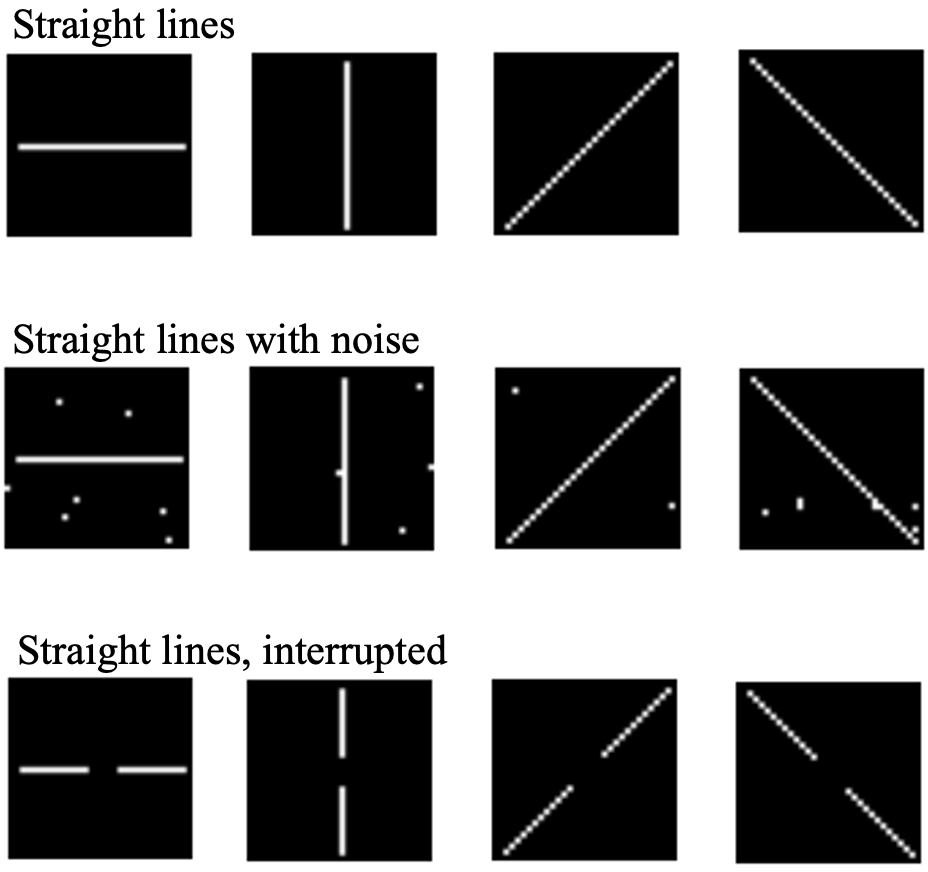
\includegraphics[width=0.59\textwidth]{straight_line_samples}
    \caption[Sample images from the dataset]{Sample images from the straight line dataset. The first row shows the images used for training, the second row shows images with noise, and the third row shows discontinuous lines. The images in the second and third rows are only used for evaluation.}
    \figlbl{straight_line_samples}
\end{figure}


The dataset is generated online, meaning images are created when required and not stored on the disk. This provides high flexibility and allows dynamically generating different images, which is helpful, especially during evaluation.
For the conducted experiments, black and white images with a dimensionality of $[1 \times 32 \times 32]$ are used, whereby $1$ is the number of colour channels and $[32 \times 32]$ is the image's width and height, respectively.
The dataset is binary and depicts different types of lines.
All background pixels are set to $0$, while the pixels representing a line are set to $1$.
No normalisation is used as the data distribution of the binary dataset is already well-aligned, and normalisation is unnecessary.

During \emph{training}, four fixed images are used, depicting vertical, horizontal, and two diagonal lines (one with a positive and one with a negative slope). The starting and ending coordinates $(x, y)$ of these lines are as follows: A horizontal line from $(2, 16)$ to $(30, 16)$, a vertical line from $(16, 2)$ to $(16, 30)$, a diagonal line with positive slop from $(2, 2)$ to $(30, 30)$, and a diagonal line with negative slop from $(2, 30)$ to $(30, 2)$. These lines are shown in the first row of \figref{straight_line_samples}.
The training dataset consists of $500$ images, randomly sampled in each epoch.

During \emph{testing}, different kinds of images are generated. 
First, an optional noise parameter is introduced. In this thesis, this parameter is set to $0.005$, letting each neuron with a probability of $0.5\%$ switch its activation from $0$ to $1$, or vice versa. Thus, on average, $5.12$ pixels in the image change their activation. Such images with noise are shown in the second row of \figref{straight_line_samples}.
Second, the continuous line is interrupted in the middle, resulting in a discontinuous line. The length of the break is a hyperparameter and within a range of $0$ to $20$ pixels. Lines with a break of $5$ pixels are shown in the last row of \figref{straight_line_samples}.
Third, a trajectory strategy generates different views of an image, as described in \secref{model_overview}. This trajectory strategy allows the specification of starting and ending coordinates and generates a set of lines encompassing all trajectories between these coordinates.
The result of such a trajectory strategy is shown in \figref{straight_line_trajectories}, where a horizontal line is converted to a diagonal line with a positive slope. Note that this strategy is only utilised during testing, as the required components to learn from different views during the training process have not yet been implemented. Therefore, this trajectory strategy generates images during evaluation that the network has not seen during training. 

\begin{figure}[h]
    \centering
    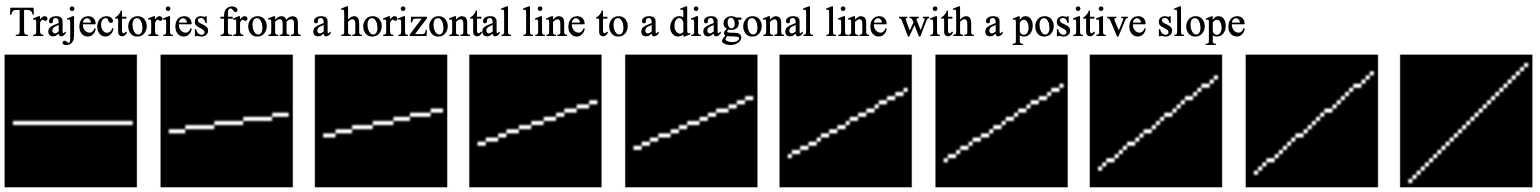
\includegraphics[width=0.99\textwidth]{straight_line_trajectories}
    \caption[Sample line trajectory strategy]{A sample trajectory strategy is applied to the horizontal line so that it becomes, over several steps, a diagonal line.}
    \figlbl{straight_line_trajectories}
\end{figure}


\section{Sensory System \emph{S0}}\seclbl{exp_s0}
The dataset used in this thesis is straightforward and does not require learning highly specialised filters.
Furthermore, it is expected that learning proper filters is a simple task that poses not many challenges as deep learning networks have proven themselves as excellent pattern recognition systems able to learn filters that are well tuned to the data domain \sidecite{bhatt_cnn_2021, bertolini_machine_2021, zou_object_2023}.

Hand-crafted filters are sufficient and preferred for the conducted experiments as they do not require additional training and can be highly interpretable. Interpretability facilitates a better understanding of the extracted features and better comprehension of the net fragments built in the subsequent stage based on these features. 

\begin{figure}[h]
    \centering
    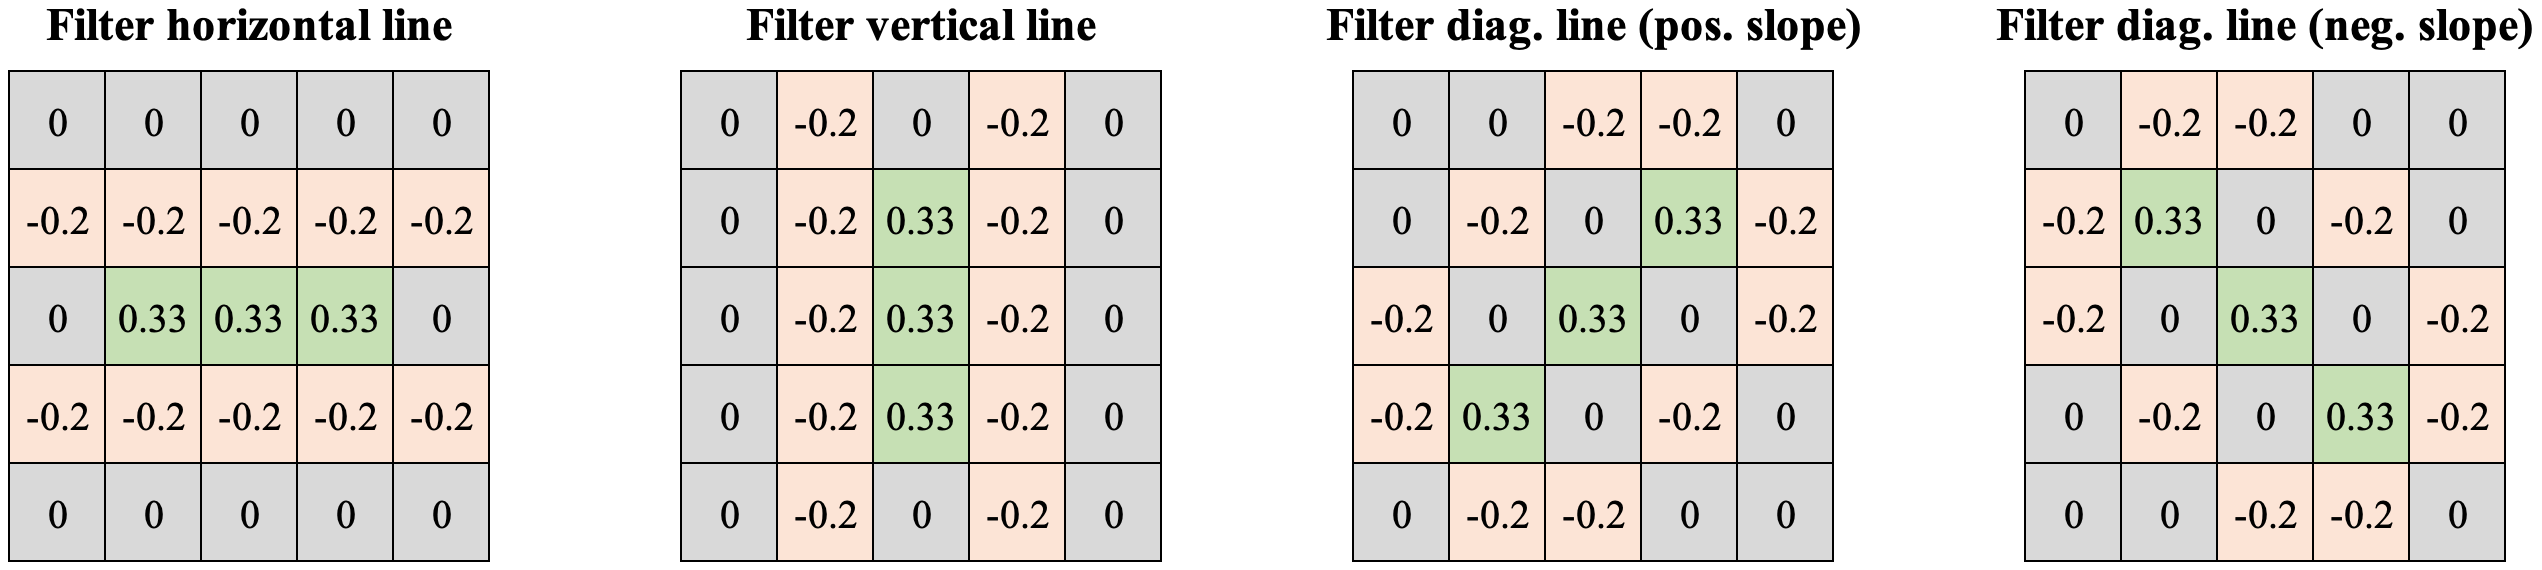
\includegraphics[width=0.99\textwidth]{filters_feature_extractor}
    \caption[Hand-crafted filters of the sensory system]{The hand-crafted filters of the sensory system are used to extract features from the images. The filters are optimised for horizontal, vertical, and diagonal lines.}
    \figlbl{filters_feature_extractor}
\end{figure}

The hand-crafted filters are illustrated in \figref{filters_feature_extractor}.
Four filters are used, each specialising in a different type of line.
These filters function similarly to a convolutional layer with frozen (non-trainable) weights and no bias term. 
During processing, the filters are shifted with a stride of $1$ across the input image of size $[1 \times 32 \times 32]$ so that it is applied at all input positions. 
The borders are padded with $0$ values to keep the input and output sizes identical.
After applying the four filters, the output has a shape of $[4 \times 32 \times 32]$. 
However, the activations can be in the range of $(-1, ..., +1)$.
In order to obtain binary activations, these activations are used as the firing probability of a Bernoulli neuron, whereby values $\leq 0$ are mapped to an activation probability of $0\%$.
This means the initial activation is used as a probability value, and its binary activation is sampled from a Bernoulli distribution.


\begin{figure}[h]
    \centering
    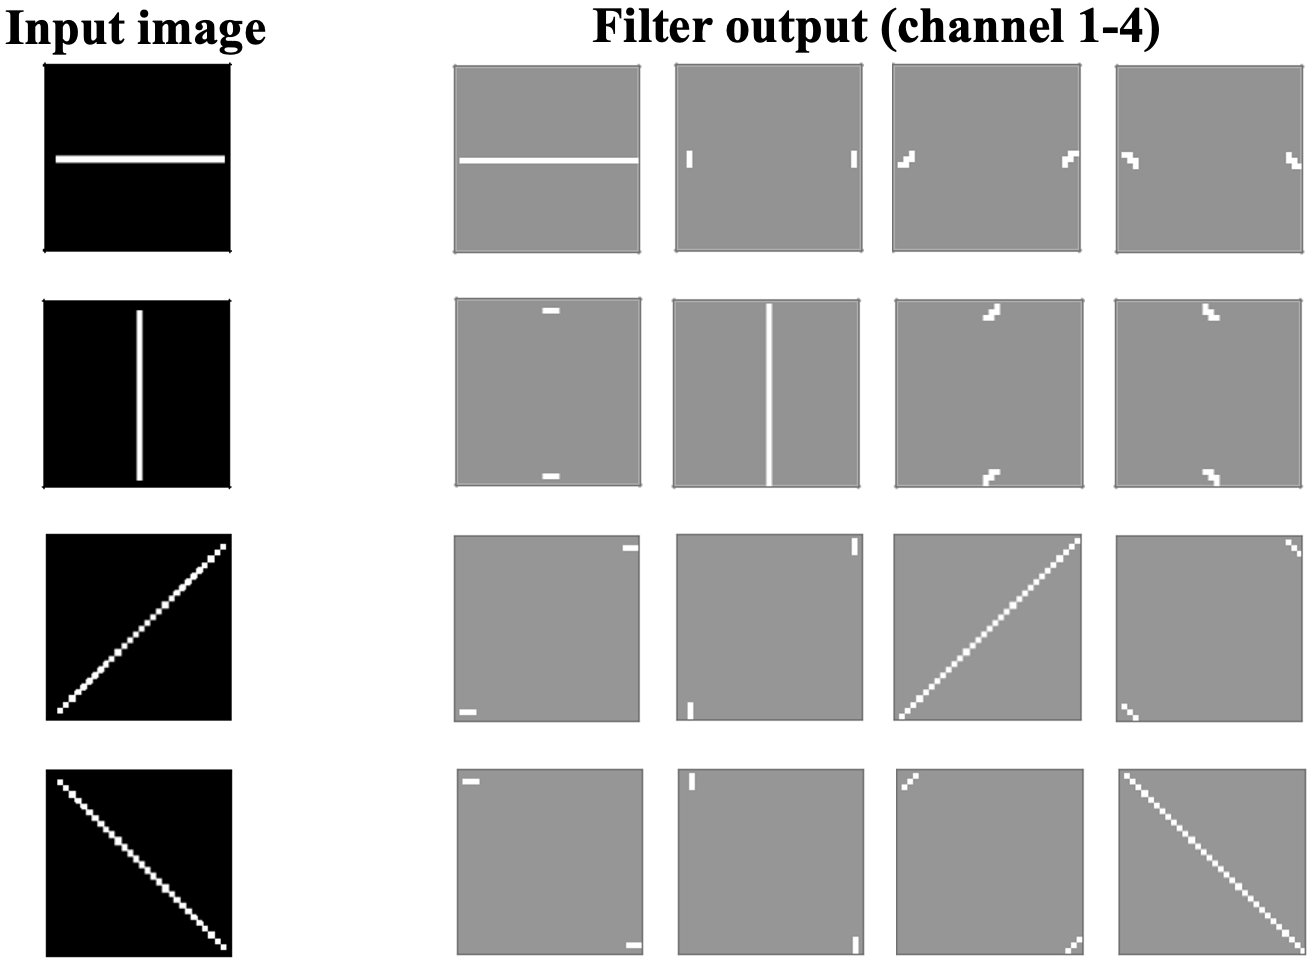
\includegraphics[width=0.99\textwidth]{results_filter}
    \caption[Output of hand-crafted filters for straight lines]{Output of hand-crafted filters for the straight lines used during training. Each row shows the input image (on the left) and the responses of the four filters (on the right).}
    \figlbl{result_filter}
\end{figure}

In \figref{result_filter}, the filter response of these four filters applied to the images from the training dataset is shown.
Please note that a fixed threshold of $0.5$ instead of a Bernoulli neuron is used to make this figure appear visually less noisy.
For each type of line, one filter specialising in this line has a strong response, almost reassembling the input image (except extending the line by a few pixels).
The other filters primarily activate around the endpoints of the lines.


\section{Feature Extracting Stage \emph{S1}}\seclbl{exp_s1}
The feature-extracting stage further processes the sensory signal of shape $[4 \times 32 \times 32]$ to build net fragments. In the conducted experiments, no alternative cells are used. As described in \secref{framework_s1}, the input of \emph{S1} consists not only of the signal from the sensory system but also of the previous net fragments that can be overridden by the feedback from the object prototypes.
These inputs are stacked along the first dimension, resulting in an input matrix of shape $[8 \times 32 \times 32]$ and an output of shape $[4 \times 32 \times 32]$.
Thereby, the first four channels (i.e. the input with index $[(1, ..., 4) \times H \times W]$) are the output of the sensory system, and the last four channels (i.e. input with index $[(5, ..., 8) \times H \times W]$) are the previous net fragments.
The previous net fragments are overridden by the feedback of \emph{S2} if the mean square error between the net fragments and the \emph{S2} feedback is below a threshold value of $0.05$, and thus, the feedback is considered credible.

The lateral support distance of a single cell is defined as $n_l=5$. Consequently, a cell can get lateral support by all cells not further away than $5$ cells in each direction or from $2n_l+1=11$ cells per input channel.
The lateral support is implemented with a convolutional kernel $\boldsymbol{W}$ of size $[4 \times 8 \times 11 \times 11]$, that maps the $8$ input channels to $4$ output channels.
The kernel is initialised as described in \secref{lateral_init} and updated with Hebbian updates as described in \secref{framework_hebb_updates}.
However, implementing Hebbian updates for a convolutional kernel is challenging, as in an efficient implementation, the kernel is not shifted over the image, but a circulant matrix is used, which cannot provide information about which cells connected through a synapse were active simultaneously \sidecite{miconi_hebbian_2021}. This is solved by using two convolutional kernels as described in \secref{exp_conv_details}. However, the principle remains the same, and this two-step procedure is only used for higher computational efficiency.

The convolutional operation is applied between the input and the weight matrix $\boldsymbol{W}$ to obtain the lateral support strength.
This support strength is normalised as described in \secref{framework_norm} using an upper cell-support limit of $\rho = 1.3 \cdot n_l$.
However, at the end of the normalisation procedure, each output channel is divided by its highest value to ensure that the support strength is in the range $(0, ..., 1)$ and the highest activation has an activation probability of $1$.
%
\begin{align}\eqlbl{exp_norm}
	x_{c_{\text{out}},w,h} := \frac{x_{c_{\text{out}},w,h}}{\max_{c=0} C_{\text{out}} x_{c,w,h}}
\end{align}
%
The input is processed over $T=6$ timesteps, and the Hebbian update is calculated between the input and the median activation during these timesteps to increase training stability.
The learning rate is set to $0.1$, the mini-batch size is $256$, and the model is trained for $10$ epochs.



\subsection{Implementation Details}\seclbl{exp_conv_details}
In an efficient implementation of a convolutional layer, a circulant matrix is used so that all kernel updates can be calculated in parallel \cite{miconi_hebbian_2021}. However, by applying this operation, information about the cell's lateral influence is lost.

This problem is solved using two convolutional operations, producing a slight memory overhead but increasing computation drastically compared to shifting kernels in a loop over the image.
The first operation is a fixed, binary convolution that restructures each input patch into a single-column vector. This is followed by a $1\times1$ convolution containing the actual weights. Specifically, the input is passed through a fixed convolution with an input size of $\left[C_{in} \times (2n_l+1) \times (2n_l+1)\right]$ and $C_{in} 2(2n_l+1)$ output channels. The weight vector for this convolution is set to $1$ for the connections linking input $c_i,w,h$ to output $c_iwh$ (where $c_i$ $w$, and $h$ range from 1 to $C_{in}$, $2n+1$, and $2n+1$, respectively), and it is set to 0 everywhere else. This process reorganises the values of each input patch from the original convolution into non-overlapping column vectors, effectively duplicating them. Next, the actual weights of the original convolution can be applied using a simple $[1\times1]$ convolution. This can be achieved by performing a tensor product with appropriate broadcasting.
Thus, the proposed method allows calculating Hebbian updates \sidecite{hebb_organization_1949} while fully leveraging the computational capabilities of current deep learning hardware.







\section{Prototype Stage \emph{S2}}\seclbl{exp_s2}
The conducted experiments focus on \emph{S1}.
However, since \emph{S2} is needed to provide feedback to \emph{S1}, a mockup simulates such a feedback signal.
The mockup described in the following is inspired by the brain's memory system \sidecite{miyashita_inferior_1993}, located in the prefrontal cortex \sidecite{tomita_top-down_1999}.
In the context of our framework, such a memory system would be located after \emph{S2} and map the reference object to memories.
A single memory can be considered a label, i.e., the projection fibres could initiate a mapping to a face while the memory is the person's name.

Many neurons are active when we see a person for the first type.
However, after a short learning period, our brain is rewired to remember a frequently occurring object with one or a few single cells \sidecite{gross_genealogy_2002}.
The proposed mockup implements this behaviour: It maps a 2D activation pattern to one or a few single cells in a self-organising manner and vice versa.
This memory mapping is directly applied to \emph{S1}, mapping net fragments to memory cells and returning feedback, thereby ignoring projection fibres.
Thus, a feedback signal is provided without implementing \emph{S2}.



\subsection{Implementation}
The mockup should map net fragments in \emph{S1} denoted as $\boldsymbol{a}$ to a hidden memory state $\boldsymbol{h}$ and vice versa. The mapping processes can be described as conditional probabilities $P(\boldsymbol{h}|\boldsymbol{a})$ and $P(\boldsymbol{a}|\boldsymbol{h})$.
Restricted Boltzmann machines (RBMs) \sidecite{hinton_training_2002, smolensky_information_1986} are generative stochastic networks that can learn such a probability distribution.
They use a linear transformation to map from $\boldsymbol{a}$ to $\boldsymbol{h}$ and the inverse linear transformation to map backwards from $\boldsymbol{h}$ to $\boldsymbol{a}$.

First, the 3D activation map containing the net fragments is flattened and multiplied with a weight matrix $\boldsymbol{W}_{S2}$ of size $\left[(C_{out}\cdot W\cdot H) \times Z\right]$. This results in a one-dimensional binary vector $\boldsymbol{h}$ of length $Z$, whereby $Z$ is a hyperparameter and defines the memory's capacity.
In the conducted experiments, the capacity is set to $Z=16$.
For both mappings $P(\boldsymbol{h}|\boldsymbol{a})$ and $P(\boldsymbol{a}|\boldsymbol{h})$, a bias term $\boldsymbol{b}_a$ and $\boldsymbol{b}_h$, and the sigmoid function to squeeze the activations in the range $(0, ..., 1)$ are used. 
The weight $\boldsymbol{W}_{S2}$ can be interpreted as fully connected projection fibres, mapping the cells in \emph{S1} ($\boldsymbol{a}$) to memory cells ($\boldsymbol{h}$).
\begin{align}\eqlbl{l2_1}
	P(\boldsymbol{h}_j=1 | \boldsymbol{a}) = \text{sigmoid}(\boldsymbol{W}_{S2} \cdot \boldsymbol{a} + \boldsymbol{b}_a) = \frac{1}{1 + e^{\boldsymbol{W}_{S2} \cdot \boldsymbol{a} + \boldsymbol{b}_a}}
\end{align}
\begin{align}\eqlbl{l2_2}
	P(\boldsymbol{a}_i=1 | \boldsymbol{h}) = \text{sigmoid}(\boldsymbol{W}_{S2}^\top \cdot \boldsymbol{h} + \boldsymbol{b}_h) = \frac{1}{1 + e^{\boldsymbol{W}_{S2}^\top \cdot \boldsymbol{h} + \boldsymbol{b}_h}}
\end{align}
Similar to \emph{S1}, the activity of these neurons is used as probability, and the binary output is sampled from a Bernoulli distribution.
\begin{align}\eqlbl{l2_3}
	\boldsymbol{h}_{out} \thicksim \text{Bernoulli}(P(\boldsymbol{h} | \boldsymbol{a}) )
\end{align}
\begin{align}\eqlbl{l2_4}
	\boldsymbol{a}_{out} \thicksim \text{Bernoulli}(P(\boldsymbol{a} | \boldsymbol{h}))
\end{align}

The parameters $\boldsymbol{W}_{S2}$, $\boldsymbol{b}_a$, and $\boldsymbol{b}_h$ are updated by minimising the difference of the free energy function $F(\cdot)$ \sidecite{hinton_training_2002} between $\boldsymbol{a}_{in}$ and $\boldsymbol{a}_{out}$ (i.e. $F(\boldsymbol{a}_{in}) - F(\boldsymbol{a}_{out})$). Recent findings suggest that the brain implements algorithms similar to minimising energy functions as well \sidecite{isomura_experimental_2023}. Since no backpropagation of error is used, this mapping seems biologically plausible as the rest of the framework. For more details about the implementation, interested readers are referred to the publication by \citeay{hinton_training_2002} or a well-written blog post by \sideciteay{hui_machine_2017}.
The free energy function is minimised using the Adam \sidecite{kingma_adam_2017} optimiser with a learning rate of $0.05$, and the parameters $\beta_1=0.9$, $\beta_2=0.999$, and $\epsilon=1\cdot 10^{-8}$.
During training, the learning rate is reduced by a factor of $0.1$ if the free energy does not reduce further for more than $2$ epochs until a final learning rate of $1\cdot 10^{-6}$ is reached.
The batch size is set to $256$, and the model is trained for $10$ epochs (similar to \emph{S1}).

By minimising the free energy function, the memory decides by itself which representation should be stored.
After observing cell activity $\boldsymbol{a}$ in \emph{S1}, $\boldsymbol{a}$ is mapped to $\boldsymbol{a}{out}$, whereby $P(\boldsymbol{h}|\boldsymbol{a})$ defines the probability for the cell activity in the memory. Since we sample $\boldsymbol{h}_{out} \thicksim \text{Bernoulli}(P(\boldsymbol{h} | \boldsymbol{a}) )$, $\boldsymbol{h}_{out}$ becomes binary and cells with a low probability tend to be turned off, while cells with a high probability tend to fire.
This can be interpreted as a filter against noise and slight deformations: A cell activity $\boldsymbol{a}$ is mapped to the closest known configuration of $\boldsymbol{h}$.
To provide feedback to \emph{S1}, the returned vector $\boldsymbol{a}_{out}$ is calculated in a similar fashion and sampled from $P(\boldsymbol{a}|\boldsymbol{h})$. Thus, the memory is a probabilistic associative memory, mapping an input to a hidden state from which an output is sampled.
This sampled output is not a reconstructed input but rather an optimised prototype stored in the memory and used to provide feedback to \emph{S1}.





